\begin{slide}

	\slidetitle{OS Abstractions Need a Privileged Kernel}

	\begin{columns}[c,onlytextwidth]
		\begin{column}{0.45\textwidth}
			\centering
			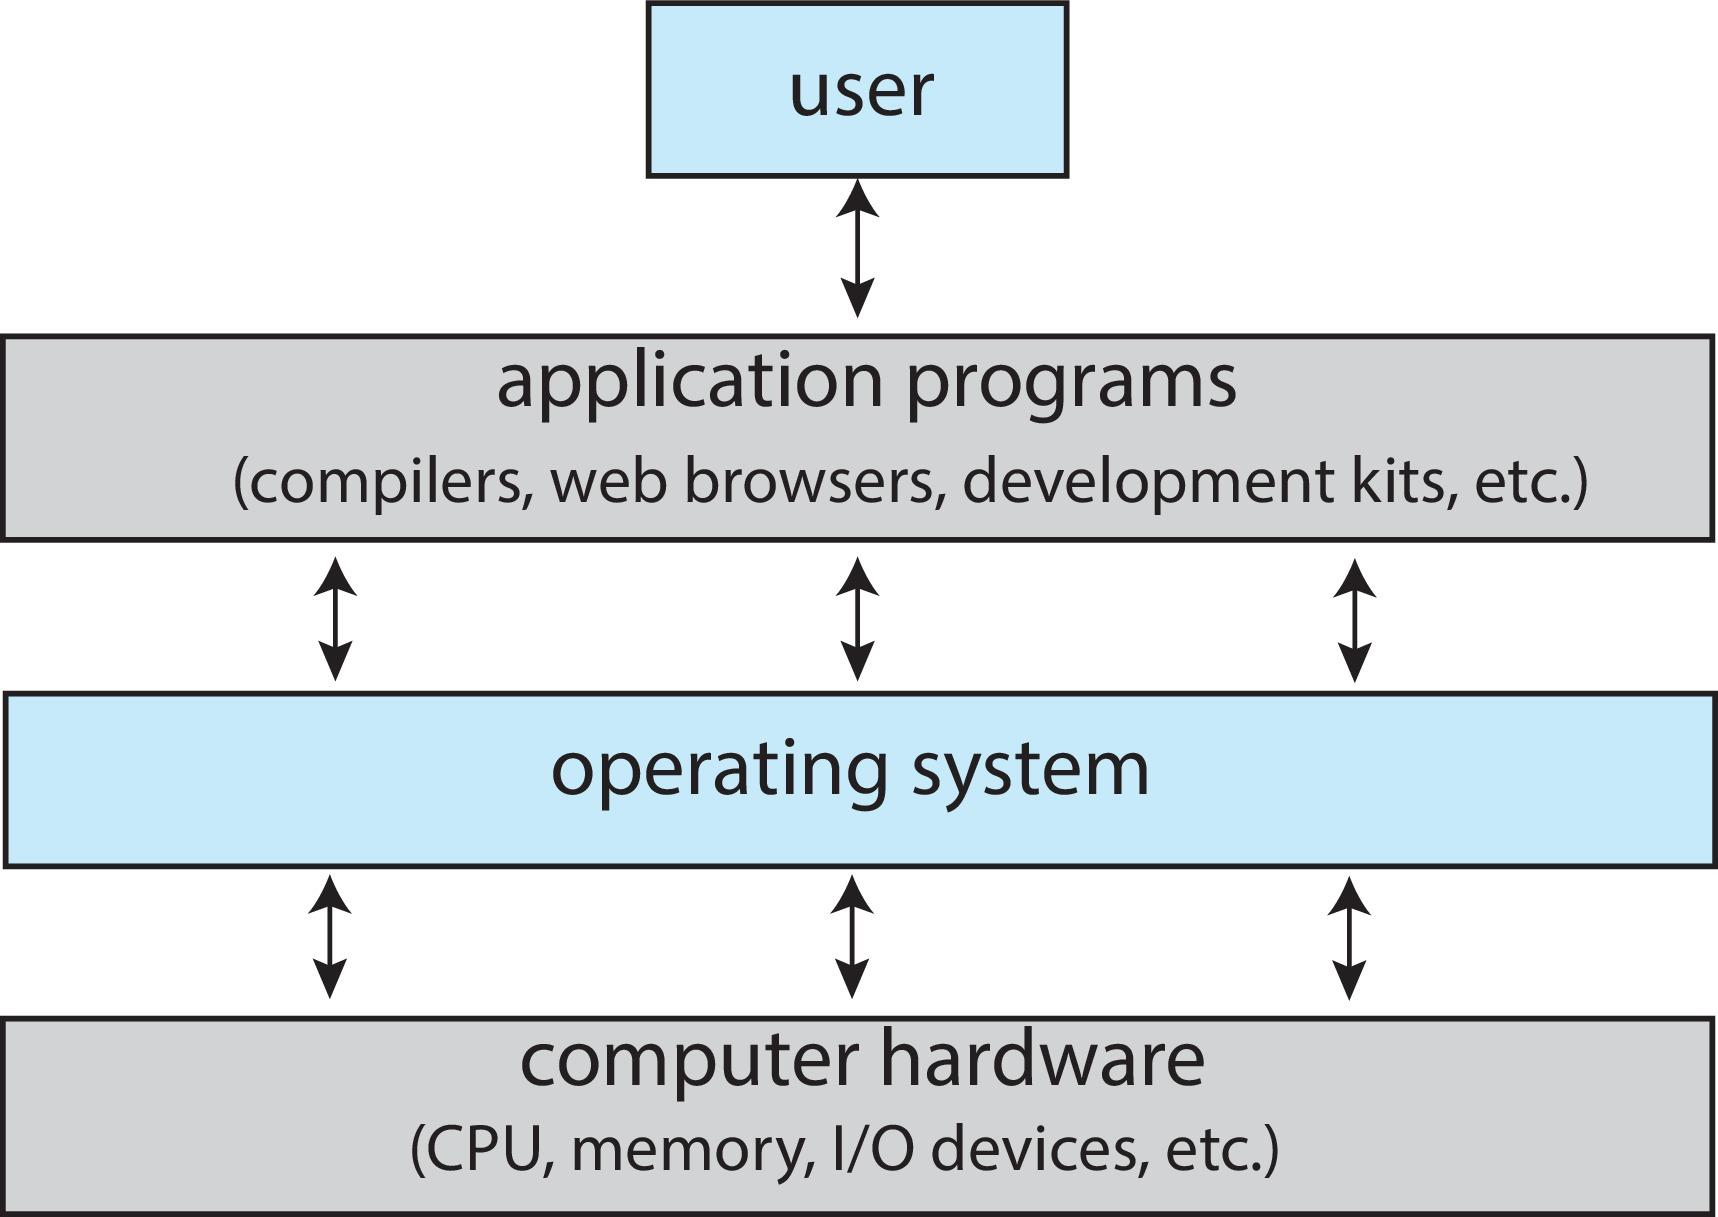
\includegraphics[width=0.82\textwidth]{components-of-a-computer.jpeg}
		\end{column}
		\begin{column}{0.51\textwidth}
			Applications cannot enforce isolation or resource sharing themselves.

			\medskip

			The \textbf{kernel} can:
			\begin{itemize}
				\item Manage shared hardware and state
				\item Enforce process isolation
				\item Decide whether requests are permitted
			\end{itemize}
		\end{column}
	\end{columns}

\end{slide}

\begin{slide}

	\slidetitle{Why Does the CPU Need Two Modes?}

	\begin{columns}[T,onlytextwidth]
		\begin{column}{0.47\textwidth}
			\textbf{User mode}
			\begin{itemize}
				\item Runs applications
				\item Restricts privileged instructions
				\item Restricts access to kernel memory
			\end{itemize}
		\end{column}
		\begin{column}{0.49\textwidth}
			\textbf{Kernel mode}
			\begin{itemize}
				\item Runs trusted OS code
				\item Can control devices and memory
				\item Can affect the whole system
			\end{itemize}
		\end{column}
	\end{columns}

	\bigskip

	The CPU enforces this boundary; an application cannot simply grant itself privilege.

\end{slide}

\begin{slide}

	\slidetitle{Most Application Instructions Stay in User Mode}

	\begin{minted}{c}
total += values[i];
	\end{minted}

	Arithmetic, branches, and access to a process's own memory execute directly in user mode.

	\bigskip

	The CPU enters kernel code only when an event requires OS involvement:

	\begin{itemize}
		\item A system call
		\item An exception
		\item A hardware interrupt
	\end{itemize}

\end{slide}

\begin{slide}

	\slidetitle{What If Applications Had Kernel Privileges?}

	If every application ran with kernel privileges, what could happen if:

	\bigskip

	\begin{itemize}
		\item A browser wrote to any memory address it chose?
		\item A game disabled the timer that lets the OS regain the CPU?
		\item Two programs issued conflicting commands to a disk?
	\end{itemize}

\end{slide}

\begin{slide}

	\slidetitle{Three Events Transfer Control to the Kernel}

	\textbf{System call}

	\leftspace an application deliberately requests an OS service

	\medskip

	\textbf{Exception}

	\leftspace the current instruction needs attention, such as a page fault or divide-by-zero

	\medskip

	\textbf{Interrupt}

	\leftspace hardware signals an event, such as a timer tick or completed device operation

	\bigskip

	The kernel handles the event, then either resumes the process or takes another action.

\end{slide}

\begin{slide}

	\slidetitle{Event 1: A System Call Is a Deliberate Request}

	\begin{minted}{c}
#include <unistd.h>

int main(void) {
    write(STDOUT_FILENO, "hello\n", 6);
    return 0;
}
	\end{minted}

	\onslide<2->

	\texttt{write()} takes a file descriptor, the address of some bytes, and a byte count.

	\medskip

	Calling it deliberately requests an OS service. The kernel performs the output and returns a result.

\end{slide}

\begin{slide}

	\slidetitle{Event 2: An Instruction Causes an Exception}

	\begin{minted}{c}
int main(void) {
    int *value = 0;
    *value = 42;
    return 0;
}
	\end{minted}

	\onslide<2->

	Dereferencing \texttt{value} has undefined behaviour in C.

	\medskip

	On a typical protected system, the CPU raises a page-fault exception. The kernel handles it, usually terminating the process with \texttt{Segmentation fault}.

\end{slide}

\begin{slide}

	\slidetitle{Event 3: An Interrupt Arrives from Hardware}

	\begin{minted}{c}
int main(void) {
    for (;;) {
        /* keep computing */
    }
}
	\end{minted}

	\onslide<2->

	In C, \texttt{for (;;)} means loop forever. The loop makes no system call and causes no exception.

	\medskip

	Timer hardware still interrupts the CPU periodically. The kernel may resume this process or schedule another one.

\end{slide}

\begin{slide}

	\slidetitle{Applications Request Kernel Services with System Calls}

	\begin{center}
		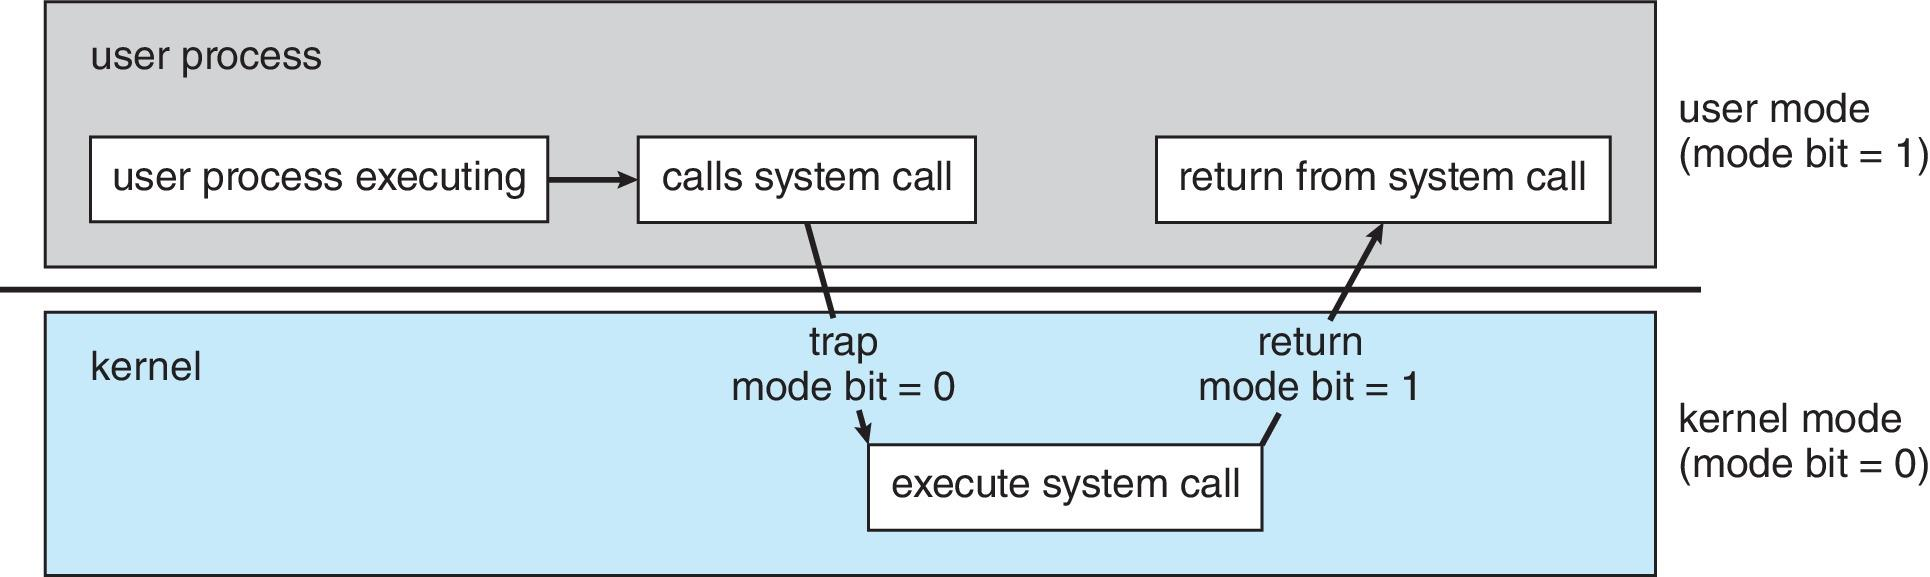
\includegraphics[width=0.72\textwidth]{user-to-kernel-mode.jpeg}
	\end{center}

	\medskip

	A \textbf{system call} transfers control to an approved kernel entry point. The kernel validates the request, performs the operation, and returns a result.

	\medskip

	System calls cover operations such as files and devices, process creation, memory mapping, and communication.

\end{slide}

\begin{slide}

	\slidetitle{A Trap Transfers Control to the Kernel}

	A \textbf{trap} is how the CPU pauses the current code and starts the correct kernel code.

	\medskip

	\renewcommand{\arraystretch}{1.05}
	\begin{tabular}{@{}>{\bfseries\raggedright\arraybackslash}p{0.20\textwidth}
	                    >{\raggedright\arraybackslash}p{0.70\textwidth}@{}}
		\multicolumn{2}{@{}l}{\textbf{During setup or boot}} \\
		Kernel & Tells the CPU where the handler starts and prepares a kernel stack \\
		CPU & Keeps this information for when a trap occurs \\[0.8ex]
		\multicolumn{2}{@{}l}{\textbf{When a trap occurs}} \\
		Trigger & A system call, exception, or interrupt occurs \\
		CPU & Pauses the current code, remembers where it stopped, enters kernel mode, and starts the handler \\
		Kernel & Saves the process state, handles the event, and decides what should run next \\
		Kernel and CPU & Restore the saved state and continue the program in user mode
	\end{tabular}

\end{slide}

\begin{slide}

	\slidetitle{A System Call Uses Software and Hardware Conventions}

	\begin{minted}{c}
ssize_t result = write(1, "Hi\n", 3);
	\end{minted}

	\textbf{API}

	\leftspace names the operation and defines its argument and result types

	\medskip

	\textbf{ABI}

	\leftspace defines the system-call number and locations of arguments and results

	\medskip

	\textbf{ISA}

	\leftspace provides the controlled entry instruction: \texttt{syscall}, \texttt{svc}, or \texttt{ecall}

\end{slide}

\begin{slide}

	\slidetitle{File Descriptors Name Per-Process Resources}

	A \textbf{file descriptor} is a small integer indexing a resource held by a process.

	\bigskip

	By convention:

	\begin{itemize}
		\item \mintinline{c}{0} is standard input
		\item \mintinline{c}{1} is standard output
		\item \mintinline{c}{2} is standard error
	\end{itemize}

	\bigskip

	A descriptor may refer to a terminal, file, pipe, device, or socket; calls such as \mintinline{c}{read()}, \mintinline{c}{write()}, and \mintinline{c}{close()} use the same abstraction.

\end{slide}

\begin{slide}

	\slidetitle{Minimal Hello World Needs Output and Exit}

	\begin{minted}{c}
ssize_t write(int fd, const void *buf, size_t count);
void exit_group(int status);
	\end{minted}


	\bigskip

	Even without the C standard library, a program needs OS services to produce output and terminate.

\end{slide}

\begin{slide}

	\slidetitle{\texttt{strace} Shows Requests to the Kernel}

	\mintinline{bash}{strace ./hello_world}

	\bigskip

	Each trace line has the form: \textbf{request(arguments) $=$ result}.

\end{slide}

\begin{slide}

	\slidetitle{A C Program Makes Different Kernel Requests}

	\begin{minted}[fontsize=\small]{console}
execve("./hello_world_c", ...)          = 0
openat(..., "/usr/lib/libc.so.6", ...) = 3
mmap(..., fd=3, ...)                    = ...
brk(...)                                = ...
write(1, "Hello world\n", 12)           = 12
exit_group(0)                           = ?
	\end{minted}

	\medskip

	A normal C program also needs work from the loader and C runtime.

\end{slide}
